\documentclass{article}
% Change "article" to "report" to get rid of page number on title page
\usepackage{amsmath,amsfonts,amsthm,amssymb}
\usepackage{setspace}
\usepackage{Tabbing}
\usepackage{fancyhdr}
\usepackage{enumerate,lastpage}
\usepackage{extramarks}
\usepackage{chngpage}
\usepackage{soul,color,alltt}
\usepackage{graphicx,float,wrapfig}
\usepackage{multirow,comment}

% In case you need to adjust margins:
\topmargin=-0.45in      %
\evensidemargin=0in     %
\oddsidemargin=0in      %
\textwidth=6.5in        %
\textheight=9.0in       %
\headsep=0.25in         %

% Homework Specific Information
\newcommand{\hmwkTitle}{Lane Assignment}
\newcommand{\hmwkClass}{}
\newcommand{\hmwkAuthorName}{Donglai\ Wei}


% Setup the header and footer
\pagestyle{fancy}                                                       %
\lhead{\hmwkAuthorName}                                                 %
\rhead{\firstxmark}                                                     %
\lfoot{\lastxmark}                                                      %
\cfoot{}                                                                %
\rfoot{Page\ \thepage\ of\ \pageref{LastPage}}                          %
\renewcommand\headrulewidth{0.4pt}                                      %
\renewcommand\footrulewidth{0.4pt}                                      %

% This is used to trace down (pin point) problems
% in latexing a document:
%\tracingall

%%%%%%%%%%%%%%%%%%%%%%%%%%%%%%%%%%%%%%%%%%%%%%%%%%%%%%%%\begin{enumerate}

% Some tools
\newcommand{\enterProblemHeader}[1]{\nobreak\extramarks{#1}{#1 continued on next page\ldots}\nobreak%
                                    \nobreak\extramarks{#1 (continued)}{#1 continued on next page\ldots}\nobreak}%
\newcommand{\exitProblemHeader}[1]{\nobreak\extramarks{#1 (continued)}{#1 continued on next page\ldots}\nobreak%
                                   \nobreak\extramarks{#1}{}\nobreak}%

\newlength{\labelLength}
\newcommand{\labelAnswer}[2]
  {\settowidth{\labelLength}{#1}%
   \addtolength{\labelLength}{0.25in}%
   \changetext{}{-\labelLength}{}{}{}%
   \noindent\fbox{\begin{minipage}[c]{\columnwidth}#2\end{minipage}}%
   \marginpar{\fbox{#1}}%

   % We put the blank space above in order to make sure this
   % \marginpar gets correctly placed.
   \changetext{}{+\labelLength}{}{}{}}%

\setcounter{secnumdepth}{0}
\newcommand{\homeworkProblemName}{}%
\newcounter{homeworkProblemCounter}%
\newenvironment{homeworkProblem}[1][Problem \arabic{homeworkProblemCounter}]%
  {\stepcounter{homeworkProblemCounter}%
   \renewcommand{\homeworkProblemName}{#1}%
   \section{\homeworkProblemName}%
   \enterProblemHeader{\homeworkProblemName}}%
  {\exitProblemHeader{\homeworkProblemName}}%

\newcommand{\problemAnswer}[1]
  {\noindent\fbox{\begin{minipage}[c]{\columnwidth}#1\end{minipage}}}%

\newcommand{\problemLAnswer}[1]
  {\labelAnswer{\homeworkProblemName}{#1}}

\newcommand{\homeworkSectionName}{}%
\newlength{\homeworkSectionLabelLength}{}%
\newenvironment{homeworkSection}[1]%
  {% We put this space here to make sure we're not connected to the above.
   % Otherwise the changetext can do funny things to the other margin

   \renewcommand{\homeworkSectionName}{#1}%
   \settowidth{\homeworkSectionLabelLength}{\homeworkSectionName}%
   \addtolength{\homeworkSectionLabelLength}{0.25in}%
   \changetext{}{-\homeworkSectionLabelLength}{}{}{}%
   \subsection{\homeworkSectionName}%
   \enterProblemHeader{\homeworkProblemName\ [\homeworkSectionName]}}%
  {\enterProblemHeader{\homeworkProblemName}%

   % We put the blank space above in order to make sure this margin
   % change doesn't happen too soon (otherwise \sectionAnswer's can
   % get ugly about their \marginpar placement.
   \changetext{}{+\homeworkSectionLabelLength}{}{}{}}%

\newcommand{\sectionAnswer}[1]
  {% We put this space here to make sure we're disconnected from the previous
   % passage

   \noindent\fbox{\begin{minipage}[c]{\columnwidth}#1\end{minipage}}%
   \enterProblemHeader{\homeworkProblemName}\exitProblemHeader{\homeworkProblemName}%
   \marginpar{\fbox{\homeworkSectionName}}%

   % We put the blank space above in order to make sure this
   % \marginpar gets correctly placed.
   }%

%%%%%%%%%%%%%%%%%%%%%%%%%%%%%%%%%%%%%%%%%%%%%%%%%%%%%%%%%%%%%



%%%%%%%%%%%%%%%%%%%%%%%%%%%%%%%%%%%%%%%%%%%%%%%%%%%%%%%%%%%%%
% Make title
\title{\vspace{0.3in}\textmd{\textbf{\hmwkTitle}}}
\date{2011.11.13}
%%%%%%%%%%%%%%%%%%%%%%%%%%%%%%%%%%%%%%%%%%%%%%%%%%%%%%%%%%%%%

\begin{document}
\begin{spacing}{1.1}
\maketitle

\section{0. Plan}
Toy Model: 
\begin{enumerate}[(1)]
\item Fixed Map
\item One Straight Road Segment
\item One Less noisy Route
\item GPS Location Observation
\end{enumerate}
Real World:
\begin{enumerate}[(1)]
\item Map is noisy $\rightarrow$ Map Refinement problem
\item Multiple Roads:
\begin{enumerate}[(a)]
\item Conjunctions constraint $\rightarrow$ inner lane before turning
\item Map Matching problem
\end{enumerate}
\item Multiple Noisy Routes $\rightarrow$ need systematic correction for some routes
\item More Dynamics: Yaw rate + Speed
\end{enumerate}


\section{1. Fixed Map, One Road, One Route, GPS Location}
{\bf Settings:}\\
Map: OSM\\
Road: Part of Beacon Street, 28 way points, 2 lanes, 9m wide\\
Route: mfallon mit 2011-08-19 18-44-12-342476 Partition 0 4.rt, 183 way points
\subsection{1.1) i.i.d-Gaussian Mixture}
{\bf Model:}\\
The car is in one of the three states \{Left Lane,Changing Lane,Right Lane\}\\
The distance from GPS Location to lane center line follows from normal distribution:\\
x=(lat,lon)$|z_x$ $\sim \sum\limits_{j=1}^{3}\delta(z_x=j)\mathcal{N}(\mu_j^x,\sigma^{2})$\\
where:\\
$z_x$ is the lane assignment of x, \\
$\mu_j^x$ is the projection of x onto lane center,\\
dist is calculated with haversine formula for the sphere\\\\
{\bf Algo:}\\
Maximum Likelihood $\leftrightarrow$ Greedy Assignment: assign each x to the nearest lane center line\\ 
{\bf Result:}\\
\begin{figure}[h]
\caption{two lane center lines calculated from the way points from OSM}
  \centering
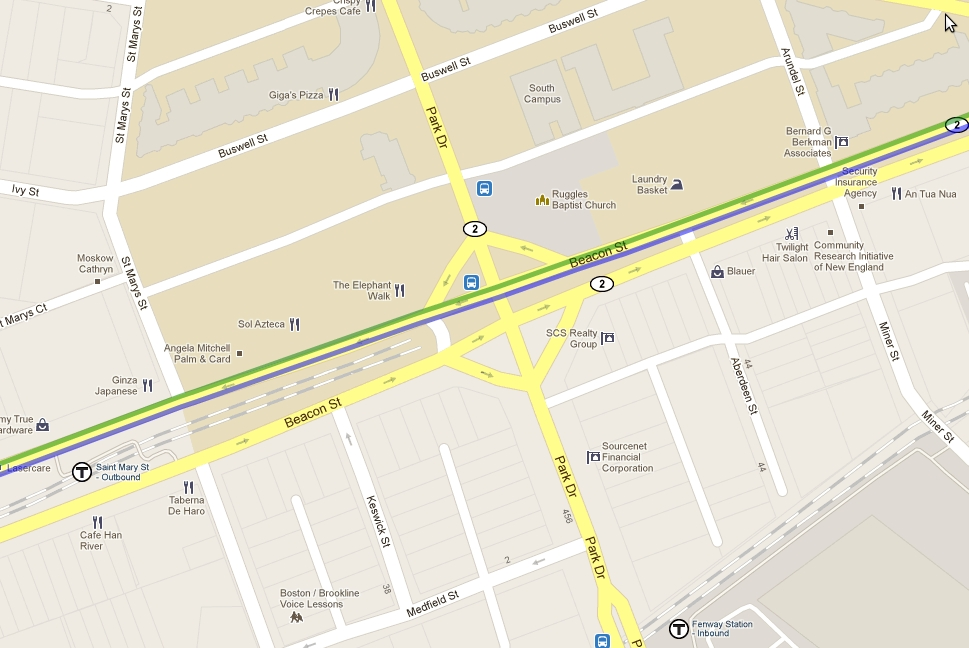
\includegraphics[width=3in,height=2in]{beacon.jpg}
\end{figure}
\begin{figure}[h]
\caption{Up: state transitions, Mid: Global look of the lane assignment, Down: Local look of the lane assignment}
  \centering
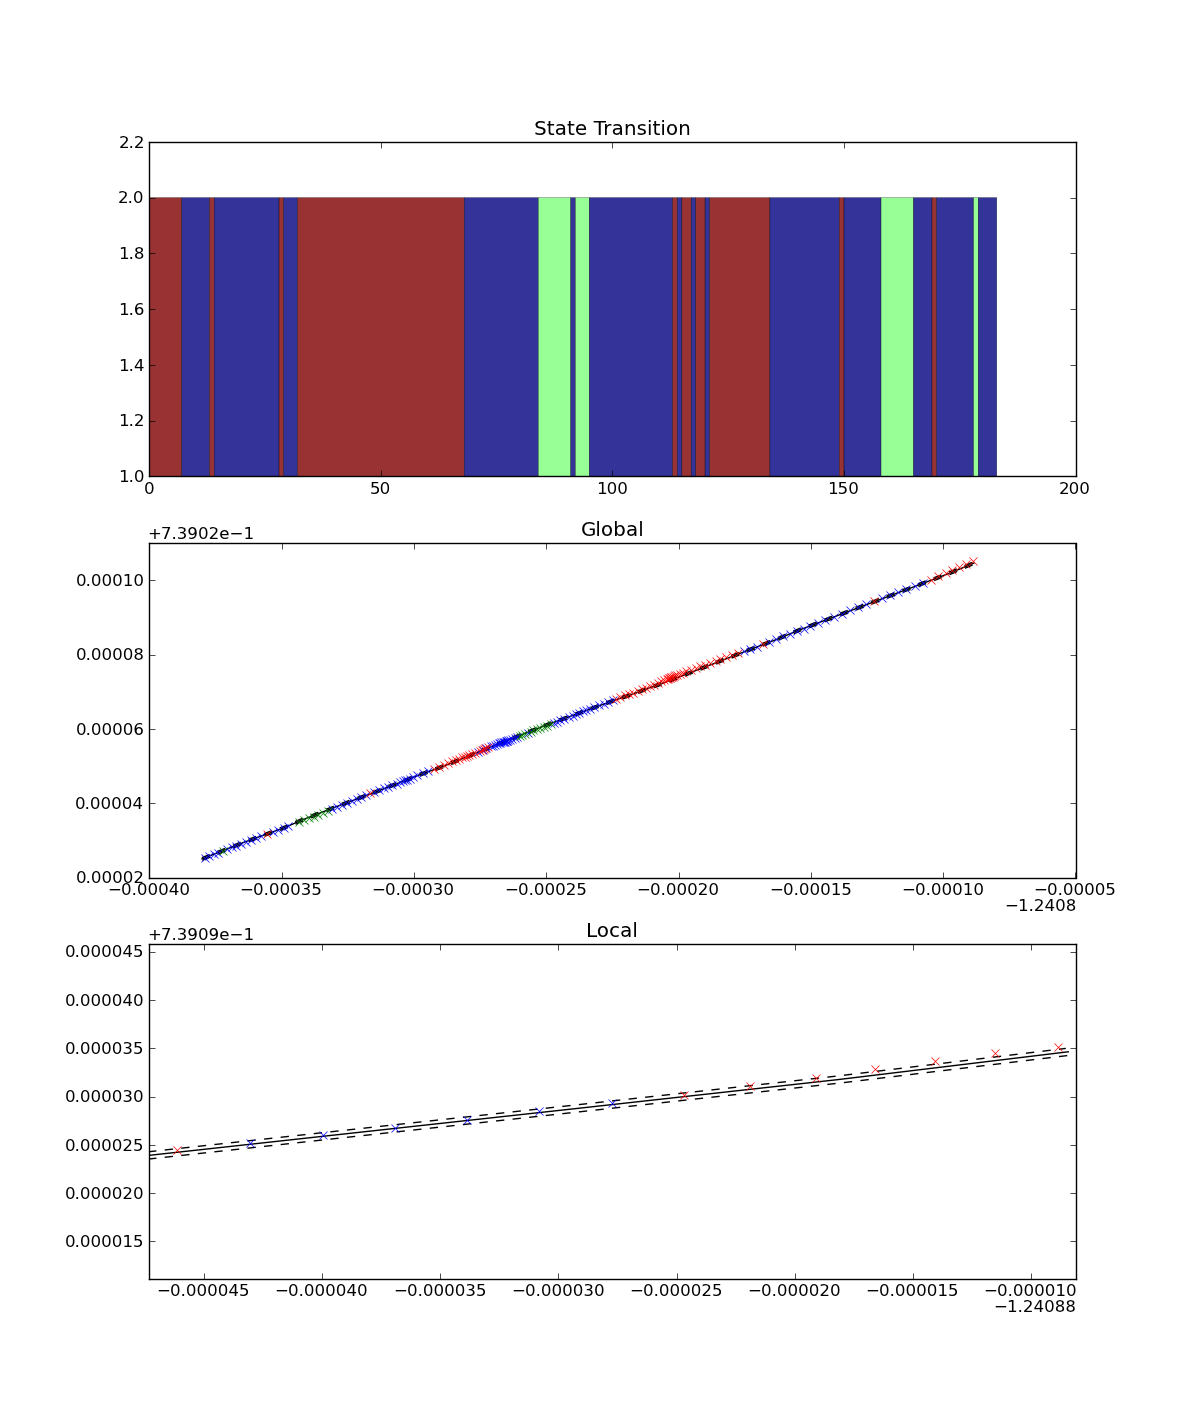
\includegraphics[width=3in,height=4in]{iid_mog.png}
\end{figure}




\subsection{1.2) Weak-Limit HDP-HMM-Gaussian Mixture}
{\bf Model:}\\
\begin{figure}[h]
\caption{Graphical Model}
  \centering
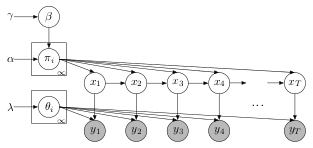
\includegraphics{gm.jpg}\\
\end{figure}
$\beta \sim Dir(\frac{\gamma}{K},...,\frac{\gamma}{K})\\
\pi_{0}| \rho \sim Dir(\rho,...,\rho)\\
\pi_{j}| \beta,\alpha \sim Dir(\alpha\beta_{1},...,\alpha\beta_{K})\\
x_{t}|\{\pi_{j}\}_{j=1}^{\infty},x_{t-1}\sim \pi_{x_{t-1}}\\
y_{t}|\{\theta_{j}\}_{j=1}^{\infty},x_{t}\sim \mathcal{N}(\mu_{x_{t}}^{y_{t}},\sigma^{2}_{x_{t}})\\
\sigma_{x_{t}}^{2}\sim \mbox{Scaled-Inv-}\chi^2(\nu_{0},\sigma_{0}^{2})\\
\mu_{x_{t}}^{y_{t}}$ is Fixed\\ \\
where $\lambda=\{\nu_{0},\sigma_{0}^{2}\},\theta_{t}=\{\mu_{x_{t}}^{y_{t}},\sigma^{2}_{x_{t}}\}$\\
{\bf Algo:}\\
Gibbs Sampler:\\\\
1) parameter:\\
Discrete Measure $\beta^{new}$:  $P(\beta^{new}|\vec x^{old},\beta^{old}) \sim Dir(\frac{\gamma}{K}+m_{1},...,\frac{\gamma}{K}+m_{K})$\\
Transition Matrix $\pi_{j}^{new}$:  $P(\pi_{j}^{new}|\vec x^{old},\beta^{new})\sim Dir(\alpha\beta_{1}^{new}+n_{j1},...,\alpha\beta_{K}^{new}+n_{jK})$\\
Initial State $\pi_{0}^{new}$: $P(\pi_{0}^{new}|x_{0}^{old}) \sim Dir(\rho+\delta(x_{0}^{old}=1),...,\rho+\delta(x_{0}^{old}=K))$\\
Covariance Matrix $\sigma^{2}_{j}$: $P(\sigma^{2}_{j}|\vec x^{old})\sim \mbox{Scaled-Inv-}\chi^2(\nu_{0}+n,\frac{\nu_{0}\sigma_{0}^{2}+(n-1)s^{2}}{\nu_{0}+n})$\\\\
where:\\
$n^{ji}$ is the number of times that transit from state j to state 1\\
$m^{j}$ is the simulated number of tables from Chinese Restaraunt Process\\
$s^{2}$ is the sample variance\\\\\\
2) state assignment:\\
Backward Sum-Product:\\
$m(x_{N}=k)=1$\\
$m(x_{n}=k)=P(y_{n+1:N}|x_{n})=\sum\limits_{x_{n+1}=1}^{K}m(x_{n+1})P(y_{n+1}|x_{n+1})P(x_{n+1}|x_{n}=k)$\\\\
Forward Sample: \\
$P(x_{1}^{new}|y_{1:N})\propto P(x_{1}^{new})P(y_{1:N}|x_{1})=\pi_{0}(x_{1}^{new})P(y_{1}|x_{1}^{new})m(x_{1})$\\
$P(x_{t}^{new}|x_{1:t-1}^{new},y_{t:N},\pi_{x_{t-1}^{new}}^{new})\propto P(x_{t}^{new}|x_{t-1}^{new})P(y_{t:N}|x_{t})= \pi_{x_{t-1}^{new}}(x_{t}^{new})m(x_{t})P(y_{t}|x_{t}^{new})$\\\\
\subsection{1.3) HSMM-Gaussian Mixture}
{\bf Result:}\\
\begin{figure}[h]
\caption{Comparison Result}
  \centering
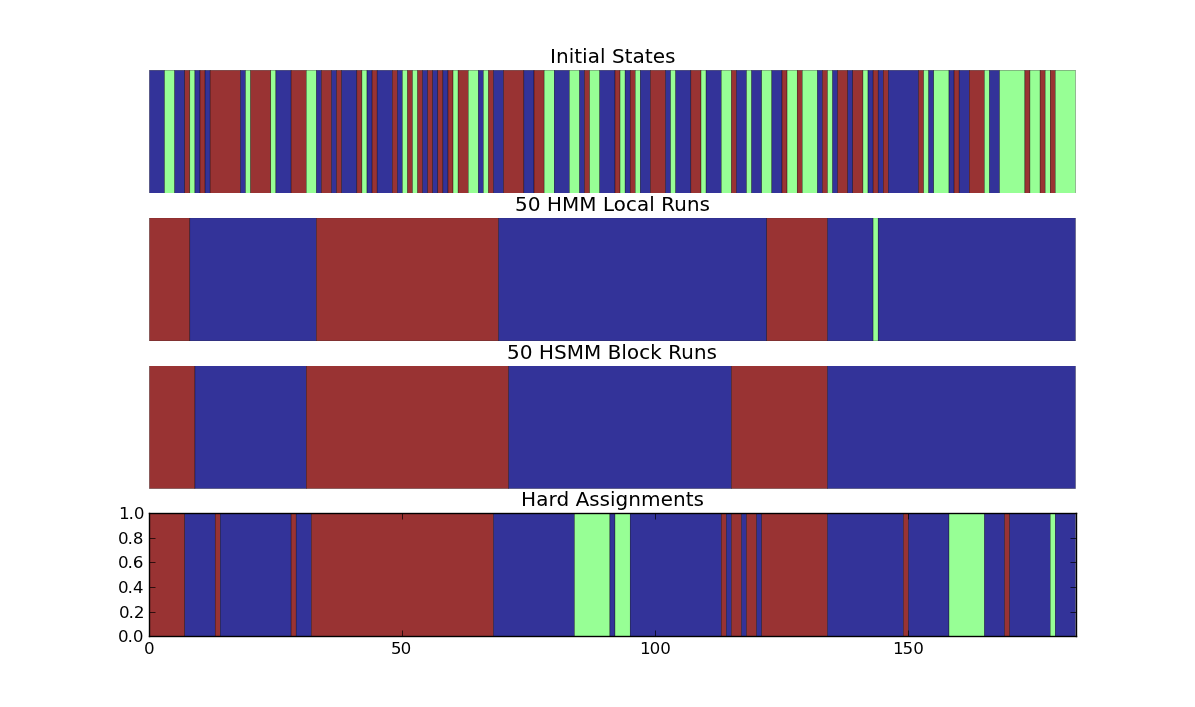
\includegraphics[width=7in,height=5in]{hsmm_mog.png}\\
\end{figure}

\end{spacing}
\end{document}

%%%%%%%%%%%%%%%%%%%%%%%%%%%%%%%%%%%%%%%%%%%%%%%%%%%%%%%%%%%%%
